\section{Measurements}
\label{sec-measurements}

In this section, we provide some measurements with respect to call and message dequeuing rates. \textit{Twilio} provides guarantees that the places calls and messages will be dequeued at a rate of 1 per sec and placed on to the phones or the browser clients [https://www.twilio.com/help/faq/twilio-basics/what-are-the-limits-on-outbound-calls-and-sms-messages-per-second - Cite this properly]. We measure the degree to which this guarantee is met. All the experiments were conducted on Lenovo W530 laptop with 8 GB RAM running on 4 cores connected to a 30 Mbps internet link.

\subsection{Calls}
\label{sec-measurements-calls}
We developed scripts that can queue automated calls to US phones and online browser clients. We queue the first call to the browser client and queue a variable number of calls to a US phone and then finally place one more call to the browser client. \textit{Twilio} deqeues the calls in the order it was placed into the queue. Using \textit{Wireshark} in the browser client, we collect the packet traces and the time stamps of the incoming call connections. We then can calculate the time difference between the first call and the second call received by the browser. A careful reader would identify that the call time stamps may not actual time when the call was dequeued from the queue and it will include the network latency involved in placing the call to the browser client. We noticed that this latency was lesser than 50 ms and so was discounted for the purpose of calculations. 

\begin{figure} \centering
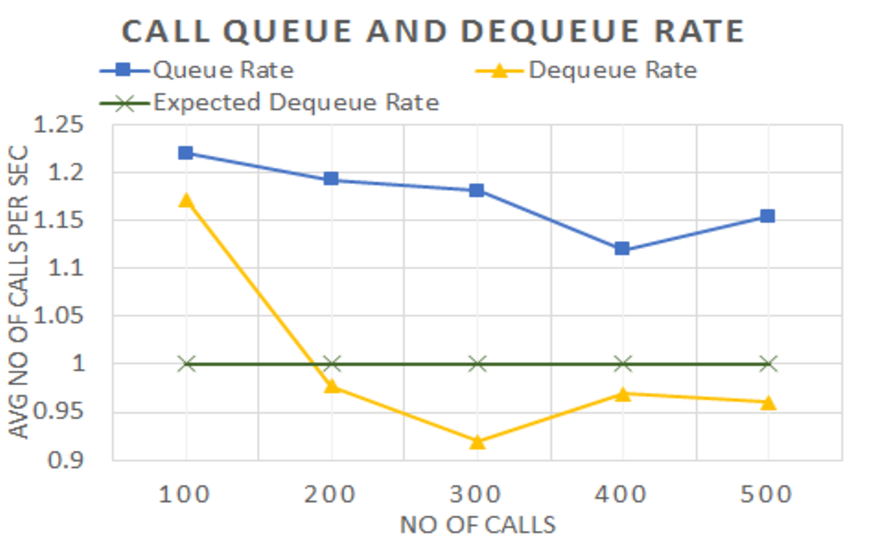
\includegraphics[width=0.45\textwidth]{graphs/calls.pdf}
\caption{\textbf{Calls queuing and dequeing.} {\footnotesize\textit{
The figure shows the queuing and dequeuing rate for calls
}}}
\label{fig:calls}
\end{figure}

Figure~\ref{fig:calls} shows the expected dequeue rate, observed dequeue rate and queue rate for calls. The horizontal axis shows increasing number of calls that we place to the phone and the vertical axis shows the queue or dequeue rate. As mentioned before \textit{Twilio} gives a guarantee to dequeue calls at the rate of 1 per second. This is shown by the flat line. We define the queue rate as the rate at which the client library can place calls into the \textit{Twilio} call queue. It is quite possible to achieve higher values of queue rate with high speed links. This value does not necessarily imply that the \textit{Twilio} server has a throttling mechanism for adding calls into the queue. The \textit{Dequeue rate} line shows the observed dequeue rate in our experiments. We notice that for a small number of calls such as 100, \textit{Twilio} dequeuing mechanism performs really well than expected. As the number of calls increases, the dequeue rate drop slightly below 1 but stays between 0.9 and 0.95. We believe that this behavior is completely acceptable if further increasing the number of calls to say few thousands. We intend to do this a future work. 

\textit{Summary}.\textit{Twilio} call dequeuing guarantees are met and exceeded for small number of calls like 100. The dequeue rate slightly falls below 1 as the number of calls increases from 100. If applications need very critical and real time data to be delivered to phones or clients, we believe it is advisable to use one Twilio number for say around 100 outgoing client/phone connections. For applications that do not need this level of accuracy at which the calls reach the clients, we believe this behavior is completely acceptable. 

\subsection{Messages}
\label{sec-measurements-sms}
We developed scripts that can queue automated messages to US phones. We queue 100 messages with varying message sizes to a sinlge US phone number. \textit{Twilio} dequeues the messages in FIFO order similar to calls. We noticed that telephone networks take a very variable amount of time to deliver messages to phones. So for calculating the dequeuing rate, we used the timestamp present in the \textit{message resource} in the \textit{Twilio} object store. We query these message resources using the REST APIs and arrive at the dequeue rate by looking at the \textit{sent timestamp} in the message resource.   

\begin{figure} \centering
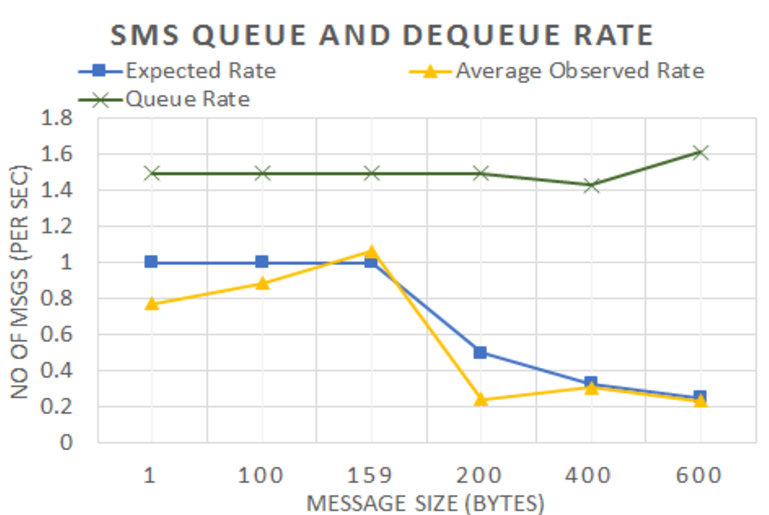
\includegraphics[width=0.45\textwidth]{graphs/sms.pdf}
\caption{\textbf{SMS queuing and dequeing.} {\footnotesize\textit{
The figure shows the queuing and dequeuing rate for messages
}}}
\label{fig:sms}
\end{figure}

Figure~\ref{fig:sms} shows the expected dequeue rate, observed dequeue rate and queue rate for SMS. The horizontal axis shows increasing size of the messages that we place to the phone and the vertical axis shows the queue or dequeue rate. As mentioned before \textit{Twilio} gives a guarantee to dequeue SMS at the rate of 1 per second. As mentioned earlier in \ref{sec-measurements-calls}, the queue rate shows the rate at which the client can push messages into the queue. It is interesting to note that the expected rate itself drops as the message size increases. \textit{Twilio} treats a single message as just 160 bytes. If the message contains say 170 bytes, \textit{Twilio} considers this as two messages and so it can queue at the rate of one message per two seconds and so the expected rate falls to 0.5 from 1. Similarly for a 400 byte message, there are three such chunks and so the expected rate drops to 0.33. It can be noted that the observed rate closely follows the expected rate. 

\textit{Summary}.\textit{Twilio} message dequeuing guarantees are well met. An interesting observation is that naive developers who do not notice the size limits of the messages may wrongly believe that \textit{Twilio} can dequeue at a rate of 1 message per second irrespective of the message size. We bring this out clearly in our study. 


